\chapter{안드로이드 프레임워크}
먼저 안드로이드 프레임워크의 소프트웨어 스택에 대한 기본적인 내용과 프레임워크 소스 활용 방안, 그리고 안드로이드 버전에 따른 이슈를 살펴보자.

\section{프레임워크 개요}
아래는 여러 안드로이드 책에도 많이 나오는 그림인데 각 스택에 대한 내용을 간단히 살펴보자.\\

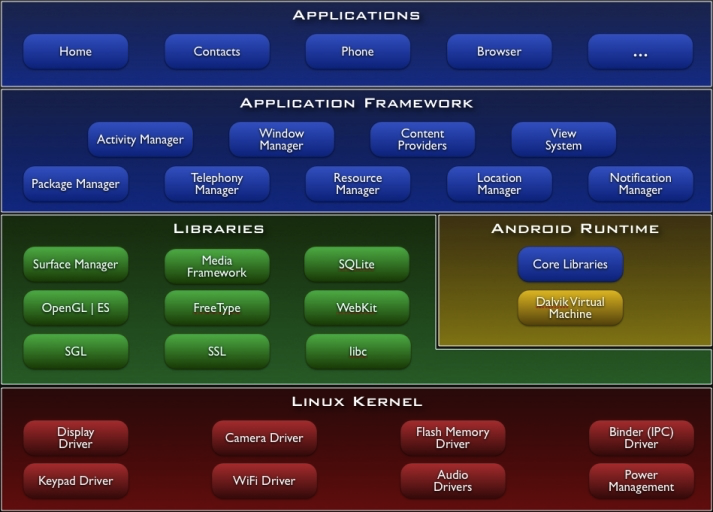
\includegraphics[scale=0.65]{system-architecture}
\begin{itemize}
\item 안드로이드에서 제공하는 기본 앱(Home, Camera, Dialer, Browser 등)과 일반 앱은 Applications 스택에 있고, Applications는 Application Framework 스택 위에서 동작한다. 기본 앱은 소스가 공개돼 있으므로 참고 자료로 활용할 수 있다. 단말 제조사들은 일반적으로 기본 앱을 커스터마이징하고, 제조사 단말에 특화된 앱도 추가로 제공한다. 요점은 단말에 깔린 기본 앱과 우리가 만드는 앱은 동일한 레벨이라는 것이다. 다만 기본 앱은 시스템 권한을 쓸 수 있다는 게 다르다.

\item Application Framework는 자바 기반의 여러 Manager가 있다. 내부적으로는 JNI를 연결해서 네이티브 C/C++로 작성된 것이 많다(Telephony Manager, Location Manager 등 주로 하드웨어 관련한 것이 그렇다). 각종 Manager는 system\_server라는 별도 프로세스에서 실행되고, 각각 시스템 서비스 형태로 있어서 앱에서는 Context의 getSystemService(String name) 메서드로 접근해서 사용한다. 별도의 프로세스에서 실행되므로 Binder IPC를 이용한 프로세스 간 통신이 필요하다.

\item Android Runtime의 Core Libraries에는 android.jar가 있다. 여기에는 android.* 패키지, com.android.* 패키지, 자바 기본 패키지(java.*, javax.*), Apache HttpClient(마시멜로에서 제거됨), DOM/SAX/XM\-LPullParser 등 자바 클래스와 안드로이드 기본 리소스(android.R)가 포함되어 있다.

\item Dalvik Virtual Machine은 자바/C/C++로 작성되어 있다(롤리팝에서는 Dalvik을 대체한 ART가 적용).\footnote{\url{https://source.android.com/devices/tech/dalvik/art.html}를 참고하자.} Register 기반의 가상 머신(Virtual Machine)으로 자바 가상 머신보다 명령이 단순하고 속도가 빠르다.
Dalvik Virtual Machine은 한 번에 여러 가상 머신 인스턴스를 띄울 수 있다. J2SE/J2EE 자바 애플리케이션을 만들다보면 여러 가상 머신 인스턴스는 당연한 얘기지만, J2ME에서는 여러 Midlet이 하나의 가상 머신에서 돌아가는 방식이었고 안드로이드에서는 이 방식을 변경하였다.

\item Libraries에는 3가지 범주의 라이브러리가 있다.\footnote{HAL(Hardware Abstraction Layer)는 별도로 나오기도 하고 Libraries에 포함하기도 한다.}
\begin{itemize}
\item Bionic이라는 커스텀 C 라이브러리(libc)\footnote{\url{http://surai.tistory.com/28}을 참고하자.}
\item WebKit/SQLite/OpenGL 같은 기능 라이브러리
\item 네이티브 시스템 서비스인 Surface Manager, Media Framework\\
/system/bin/surfaceflinger와 /system/bin/mediaserver 프로세스로 각각 실행된다.
\end{itemize}

\item 안드로이드는 리눅스 커널을 기반으로 불필요한 것은 제거하고(X-Window, glibc, 표준 리눅스 유틸리티 일부 등) 확장 패치한 것이다(Binder, Ashmem, Low Memory Killer 등).\\
이 가운데 Binder IPC는 프로세스 간 통신에 사용하는 방식이다. 
Binder에서 많이 혼동되는 게 Binder IPC(Inter Process Communication)와 Binder RPC(Remote Procedure Call)라는 두 용어인데, IPC는 하부 메커니즘이고 RPC는 IPC의 용도(리모트 콜)이다. 우리가 만드는 컴포넌트 가운데 Service와 ContentProvider는 Binder를 통해서 다른 프로세스에서 접근할 수 있는 것이다. 앱 프로세스에서 Binder Thread라는 네이티브 스레드 풀이 있고(16개까지 생성), 다른 프로세스에서 접근할 때는 이 스레드 풀을 통해서 접근한다.
DDMS에서 보면 Binder\_1, Binder\_2와 같은 이름의 스레드가 바로 Binder Thread에 속한 것이다. 

\end{itemize}
% 안드로이드 SDK는 Java 프로그래밍 언어를 사용하여 안드로이드 플랫폼 상의 애플리케이션 개발에 필요한 API들과 도구들을 제공한다.(kandroid)
\section{프레임워크 소스}
4.X 이상 버전은 Android SDK Manager를 이용해서 Sources for Android SDK를 선택해서 자바 소스를 다운로드할 수 있고, IDE에서 소스를 연결해서 보는 경우에 유용하다. 
2.X 버전의 소스를 확인하거나 네이티브까지 소스를 확인하려면, \url{https://android.googlesource.com}에서 관련 소스를 다운로드하면 된다.\footnote{\url{http://source.android.com/source/downloading.html}을 참고하자.} 참고로 3.X 허니콤 소스는 공개되어 있지 않다. 
3.X는 태블릿 전용 버전이고, 소스가 공개되어 이 버전이 폰에 이식된다면 파편화 문제가 심각해질 우려가 있어서 비공개로 결정되었다고 한다.
커널 소스는 \url{https://source.android.com/source/building-kernels.html}을 참고해서 별도로 다운로드한다.\\
 
프레임워크 소스를 다운로드하는 곳으로 \url{http://github.com/android}도 있는데, 여기는 읽기 전용 미러링 GitHub 계정이다. 항목별 소스 다운로드나 웹브라우저로 소스 보기에는 더 편리하다는 장점이 있다.\\

커널을 제외하고 소스 다운로드 결과는 아래와 같다.

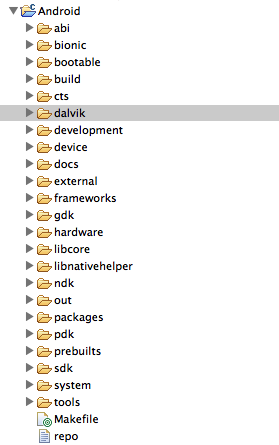
\includegraphics[scale=0.7]{sourcetree}

여기서 주요 디렉터리만 살펴보도록 하자.
\begin{itemize}
\item frameworks : 안드로이드 프레임워크. android로 시작하는 자바 패키지 포함
\item libcore: 자바 core 패키지 포함
\item system : 안드로이드 init 프로세스
\item packages : 안드로이드 기본 애플리케이션
\item bionic: 안드로이드 표준 C 라이브러리
\item dalvik: 달빅 가상 머신
\item cts: 안드로이드 호환성 테스트 관련
\item build: 빌드 시 사용
\end{itemize}

개발 시에 소스를 버전별로 모두 다운로드하지는 않고, 보통 프레임워크 소스는 
\url{http://grepcode.com}에서 확인하기도 한다. 링크가 잘 되어 있고 버전별로 차이를 확인해 볼 수도 있다.\\

개발하다가 궁금한 게 있을 때, 프레임워크 소스에서 확인하지 않고 \href{http://stackoverlow.com}{Stack Overflow}에 의존하는 경향을 가진 이들도 있다. % 면접에서 이런 분을 보기도 했다.
Stack Overflow에는 다양한 수준과 경험을 가진 사람들이 있어서 답변들이 어느 것이 맞는지 모호하기도 하고, 정작 내가 원하는 답은 없을 때도 있다.
Stack Overflow에서 답변을 찾았다고 해도 그게 맞는 것인지 검증하려면 테스트를 수행하고 프레임워크 소스로 재차 검증하는 것이 좋다.\\

예를 들어보자.
ListView의 아이템 레이아웃에 CheckBox가 있으면 ItemClick이 정상적으로 동작하지 않는다. 이런 내용은 책이나 강의에는 잘 안 나오기 때문에 처음 겪을 때 당황하게 된다. 
StackOverflow에서 검색해보면 아이템 레이아웃의 CheckBox 속성에서 android:focusable=``false''로 하라고 나온다. 이 상태에서 어쨌든 문제가 해결된다.
그런데 다른 ListView의 아이템 레이아웃에 ImageButton이 추가되었는데 또 ItemClick이 동작하지 않는다. 다시 검색을 해본다. 이런저런 얘기가 많은데 명확한 답변이 잘 안 보인다(그 가운데 물론 답이 있다). 역시 android:focusable=``false''를 써보지만 해결되지 않는다. 이때 2가지를 찾아봐야 한다. 
\begin{enumerate}
\item focusable 속성이 ListView의 OnItemClickListener에 주는 영향이 있는가? focusable 속성으로 문제가 해결되지 않으니 다른 조건이 더 있을가?
\item ImageButton의 문제가 있을까?
\end{enumerate}

먼저 ListView의 OnItemClickListener에 View의 focusable 속성이 주는 영향을 찾아보자. setOnItemClickListener() 메서드는 ListView의 상위 클래스인 AdapterView에 있다. 
여기에서 OnItemClickListener를 사용하는 위치를 찾아보면 performItemClick() 메서드이고, 또 다시 호출 위치를 따라가보면 AbsListView의 onTouchUp() 메서드에서 Child View의 hasFocusable() == true일 때는 클릭이 동작하지 않는 것을 볼 수 있다. Child View의 다른 조건은 보이지 않는다.\\

이제 CheckBox의 focusable 기본값은 어디에 있을까? 이 값은 style에 지정되어 있다.
CheckBox의 style은 /frameworks/base/core/res/res/values/styles.xml\footnote{<sdk>/platforms/android-XX/data/res 아래에서도 볼 수 있다.}에서 ``Widget.CompoundButton.CheckBox''를 보면 된다.\footnote{CheckBox 소스를 보면 defStyleAttr 파라미터 자리에 com.android.internal.R.attr.checkboxStyle이 있다. attrs.xml을 보면 checkboxStyle에 reference로 지정되어 있는데 다른 곳에서 정의한다는 의미이다. 결국 themes.xml에서 보면 ``@style/Widget.CompoundButton.CheckBox''로 다시 정의된 것을 볼 수 있다.}
parent를 쓰지 않고서도 속성을 상속하는 암묵적 상속이 있는데, 바로 CheckBox의 style은 ``Widget.CompoundButton'' style을 상속한다. 여기서 android:focusable 속성이 true로 되어 있다.
따라서 레이아웃에서 CheckBox 속성을 android:focusable=``false''로 하면 style이 다시 오버라이드되어 ListView에서 정상적으로 ItemClick이 동작한다.\\

ImageButton의 경우는 android:focusable=``false''가 반영이 되지 않는데, 그 이유는 ImageButton 생성자에서 setFocusable(true)을 실행해서 레이아웃의 속성을 다시 오버라이드하기 때문이다. 따라서 ListAdapter의 getView() 메서드에서 ImageButton에 setFocusable(false)를 실행해서 또다시 오버라이드하면 ItemClick 이 문제없이 동작한다.\\

프레임워크 리소스에서 styles.xml을 보면 CheckBox, RadioButton, ToggleButton, Switch, SeekBar, EditText, ImageButton 등 위젯의 android:focusable 속성이 true이다. 이런 위젯이 ListView에 포함된다면 주의해야 한다.
ListView의 각 아이템 레이아웃은 일반적으로 ViewGroup이고 그 안에 focusable 위젯을 가지고 있다면 다른 방법도 가능하다. 바로 ViewGroup 레이아웃 속성에 android:descendantFocusability=``blocksDescendants''를 넣으면 된다. 이 속성은 ViewGroup의 hasFocusable() 메서드에서 체크하고 있다.\\

요점은 검색만으로 문제를 해결하고 왜 그런지를 모른다면 ListView에서 CheckBox나 ImageButton은 각각의 Tip으로만 남고 까먹기도 쉽다. 프레임워크 소스 레벨에서 검증해보면, 다음에 비슷한 문제를 맞닥뜨려도 어디서부터 문제를 찾으면 되는지 알 수 있다.\\

프레임워크 소스는 각 단말 제조사에서 커스터마이징하는 경우가 많아서 예외 스택의 라인 번호가 차이가 있어 스택을 가지고 문제 위치를 쉽게 찾지 못한다. 이 때문에 프레임워크 소스를 그대로 사용하는 레퍼런스 폰인 Nexus 시리즈를 개발에 활용하는 것은 많은 도움이 된다. 앱 프로세스 내부에서 실행되는 클래스에 대해서는 디버깅 모드에서 Breakpoint를 잡아서 값을 확인할 수 있다.\\

안드로이드 내부 구조를 다 파헤쳐볼 것도 아닌데, 전체 프레임워크 소스를 다운로드할 필요가 있을까 싶다. 필자의 경우에도 다운로드하는 걸 망설였지만, 다운로드하고서 많은 도움이 되었다. C/C++ 소스까지 깊이 이해하지는 않아도 대략이라도 내부 구조를 알 수 있고, 특히 앱의 크래시 문제를 해결하는 데 쓸모가 있다. 
안드로이드 동작 방식에 대한 이해와 경험으로 문제를 크래시를 해결하는 경우가 많지만, 실제 개발에서 크래시가 코어 자바 쪽에서 생기는 경우도 있다.
아래와 같은 에러를 보게 된다면 원인을 어떻게 찾을 것인가. 두 번째 에러는 현장에서 수많은 크래시를 발생시킨 것이다.
\begin{lstlisting}[frame=single]
Caused by: java.lang.NullPointerException
	at java.text.SimpleDateFormat.parse(SimpleDateFormat.java:1004)
	at java.text.DateFormat.parse(DateFormat.java:624)
	....
\end{lstlisting}

\begin{lstlisting}[frame=single]
Caused by: java.lang.ArrayIndexOutOfBoundsException: length=2; index=2
	at java.util.regex.Matcher.group(Matcher.java:358)
	at java.util.regex.Matcher.appendEvaluated(Matcher.java:138)
	at java.util.regex.Matcher.appendReplacement(Matcher.java:111)
	at java.util.regex.Matcher.replaceFirst(Matcher.java:304)
	at java.lang.String.replaceFirst(String.java:1793)
	....
\end{lstlisting}

안드로이드에서 사용하는 코어 자바 라이브러리는 JDK에서 자바 소스를 찾으면 안된다. 
코어 자바 라이브러리는 Apache Harmony를 기반으로 만든 것이다.\footnote{안드로이드 N에서는 Open JDK 기반으로 변경된다고 한다.} 2011년도에 Apache Harmony는 종료되었지만 안드로이드에서는 이후에도 조금씩 업데이트하고 있다. 
코어 자바 소스는 /libcore/luni/src/main/java 디렉터리 아래에서 찾고 해당 라인 위치에서 원인을 찾아서 해결해야 한다.  
libcore는 기반이 되는 자바 버전이 바뀌기 전에는 거의 변경되지 않으므로, 한 버전을 다운로드해서 여러 버전에서 참고해볼 수 있다. 프로요까지 자바5, 킷캣까지는 자바6, 현재 최신 버전은 자바7 기반이다.

\section{안드로이드 버전}
안드로이드는 버전에 따라 차이가 많기 때문에, 내용 설명에서 안드로이드 버전을 가지고 얘기하는 경우가 많다. 
표로 먼저 정리해놓고 내용에서 참고하도록 하자. 굳이 본문에서 언급되지 않는 하위 버전은 표에서 제외하였다.\\

\begin{tabular}{|c|c|c|}\hline
코드네임 & API 레벨 & 안드로이드 버전 \\ \hline
프로요 & 8 & 2.2 \\ \hline
진저브레드 & 9 & 2.2\\ \cline{2-3}
 & 10 & 2.3\\ \hline
허니콤 & 11 & 3.0\\ \cline{2-3}
 & 12 & 3.1\\ \cline{2-3}
 & 13 & 3.2\\ \hline
ICS(아이스크림 샌드위치) & 14 & 4.0-4.0.2\\ \cline{2-3}
 & 15 & 4.0.3-4.0.4\\ \hline 
젤리빈 & 16 & 4.1\\ \cline{2-3}
 & 17 & 4.2\\ \cline{2-3}
 & 18 & 4.3\\ \hline
킷캣 & 19 & 4.4-4.4.2\\ \cline{2-3}
 & 20 & 4.4.3-4.4.4\\ \hline  
롤리팝 & 21 & 5.0\\ \cline{2-3}
 & 22 & 5.1\\ \hline 
마시멜로 & 23 & 6.0\\ \hline 
\end{tabular}\\

코드네임과 API 레벨이 일대일 매핑되지 않고, API 레벨과 안드로이드 버전도 마찬가지로 매핑되지 않아서 혼동되는 경우도 많다. 안드로이드 버전의 앞자리 숫자가 바뀌는 11(허니콤), 14(ICS), 21(롤리팝), 23(마시멜로)는 기억하도록 하자.
이 책에서는 설명에서 주로 코드네임으로 언급하고, 한 코드네임 안에서 여러 API 레벨이 있는 경우 구분이 필요할 때 API 레벨까지 언급하기로 한다. 
여러 API 레벨이 있는데 코드네임만 언급하는 경우는 가장 낮은 API 레벨부터 해당하는 경우이다. 이를테면 허니콤이라고 하면 API 레벨 11 안드로이드 3.0을 얘기한다.\\

각 버전의 히스토리를 알기 위해서는 아래 링크를 보자.
\begin{itemize}
\item \url{https://en.wikipedia.org/wiki/Android_version_history}
\item \url{http://socialcompare.com/en/comparison/android-versions-comparison}
\end{itemize}
아래와 같이 공식적인 링크가 있지만 최신 버전 위주로 정리되어 있고 한 번에 보기에 편하지 않다.
\begin{itemize}
\item \url{https://www.android.com/history/}
\item \url{http://developer.android.com/intl/ko/about/dashboards/index.html}
\end{itemize}

\subsection{호환성 모드}
앱이 동작하는 안드로이드 버전을 지정하기 위해서는 AndroidManifest.xml에서 uses-sdk 항목에  android:min\-SdkVersion과 android:targetSdkVersion에 버전을 기재한다. 
만든 지 오래된 앱에서 minSdkVersion만 지정하고 targetSdkVersion을 지정하지 않은 것을 본 적이 있는데, targetSdkVersion를 명시하지 않으면 minSdkVersion와 동일한 값으로 지정된다.
targetSdkVersion는 반드시 지정하도록 하자. 해당 버전까지는 테스트해봤는데 앱 실행에 문제가 없다는 의미이고, 그 버전까지는 호환성 모드를 쓰지 않겠다는 뜻이다.\\

호환성 모드는 안드로이드 버전이 올라가더라도 앱의 기존 동작이 바뀌는 것을 방지하기 위한 것이다.
프레임워크 소스를 보면 targetSdkVersion을 가지고 체크하는 부분이 있다.
\footnote{\url{http://androidxref.com}에서 버전을 선택하고 Symbol에서 targetSdkVersion을 쓰고 검색하면 확인할 수 있다.}\\

버전에 따라서 기존 동작이 변경되고 호환성 모드로 동작하는 건 어떤 게 있을까? 몇 가지 예를 들어보자.
\begin{itemize}
\item AsyncTask에서 태스크를 실행하면 허니콤 이후로 병렬 실행이 아닌 순차 실행으로 변경되었다. 이것도 targetSdkVersion이 10이하이면 안드로이드 버전이 4.X 대라고 해도 기존과 동일하게 병렬 실행으로 동작한다. ScrollView, ListView나  ViewPager에서 현재 화면의 데이터를 가져올 때 AsyncTask를 통해서 가져온다면, 순차 실행으로는 적합하지 않다. 이때는  AsyncTask를 사용하지 않고 관련한 용도의 다른 라이브러리(네트워크 용도라면 Volley 등)를 사용하거나, AsyncTask를 버전에 따라 다르게 동작하도록 코드를 작성해야 한다.\\

아래는 support-v4에 포함된 AsyncTaskCompat을 간략히 한 것이다.
\begin{lstlisting}[frame=single]
	public static <Params, Progress, Result> AsyncTask<Params,
			Progress, Result> executeParallel(
            AsyncTask<Params, Progress, Result> task, Params... params) {
        if (task == null) {
            throw new IllegalArgumentException("task can not be null");
        }
        if (Build.VERSION.SDK_INT >= 11) {
            task.executeOnExecutor(AsyncTask.THREAD_POOL_EXECUTOR, params);
        } else {
            task.execute(params);
        }
        return task;
    }
\end{lstlisting}
모든 버전에서 병렬 실행을 위해서 별도 메서드를 만든 적이 있었는데, AsyncTaskCompat을 바로 사용하도록 하자.

\item 메인 스레드 상에서 네트워크 통신이 진저브레드 API 레벨 9까지는 허용되었으나, 그 이후에는 에러를 발생시킨다. targetSdkVersion을 높여서 NetworkOnMainThreadException이 발생한다면, 백그라운드 스레드에서 네트워크 통신을 하도록 변경해야 한다.
\item 하드웨어 가속(Hardware Acceleration)은 View에서 Canvas에 그리는 모든 작업을 GPU를 가지고 하는 것이다. 하드웨어 가속은 허니콤에서 처음 시작되었고 targetSdkVersion 14 이상에서는 디폴트 옵션이다. 하드웨어 가속을 사용할 때 눈에 띄는 속도 향상은 SlidingPaneLayout이나 여러 Sliding Menu 라이브러리에서 애니메이션 시 끊김 현상이 없다는 것이다. 
필자의 경우도 애니메이션 끊김 현상이 단지 하드웨어 가속만으로 해결되는 경우를 여러 번 겪었다.
그래서 가능하면 하드웨어 가속을 쓰는 게 좋지만 항상 속도가 향상되는 것은 아니다. \url{http://developer.android.com/intl/ko/guide/topics/graphics/hardware-accel.html}을 참고해서 테스트하고 수준별(Application, Activity, Window, View)로 오버라이드하는 방법을 사용하자.
\item targetSdkVersion 14 이상에서는 App Widget에서 기본 패딩이 존재한다. 기존에는 셀의 사이즈를 꽉 채웠지만 targetSdkVersion이 올라가면 기본 패딩 때문에 App Widget의 실제 사이즈는 기존보다 작아진다. 관련해서 \ref{subsubsec:icspadding}절에 더 상세하게 설명하였다.
\item targetSdkVersion 21 이상에서는 startService()나 bindService()를 실행할 때 명시적 인텐트를 사용해야 한다.
\end{itemize}


결론적으로 단말 버전에 따라 최신 기능을 쓸 수 있기 때문에 targetSdkVersion은 높여서 쓰는 것이 권장된다. 다만 targetSdkVersion을 높일 때는 테스트할 내용이 많다.

\begin{comment}
시스템의 DPI가 낮게 변경되는 건, 안드로이드가 대화면 장치(xlargeScreens)에서 
minSdkVersion이 낮은 앱을 호환성 모드로 실행하기 때문이라고 합니다.
  
\

이해하려고 읽는 김에 Best Practice - Screen Compatibility Mode를 정리하다가, 후반엔 듬성듬성 번역해 봤습니다.
http://developer.android.com/guide/practices/screen-compat-mode.html 
 
 
Screen Compatibility Mode

 
* 안드로이드 3.0 이전에 개발된 앱이 고dpi, 고dp 화면에서 너무 작게 보이는 현상을 방지하기 위한 모드.

호환모드 상태일 때:

호환모드를 사용하지 않을 때:


버전 1.6 부터 안드로이드는 다양한 화면 사이즈를 지원했다.
하지만, 앱이 Supporting Multiple Screens의 가이드를 잘 따르지 않았다면, 대형 화면에서 문제가 발생할 수 있다.
문제를 겪는 앱을 위해, 화면 호환성 모드가 개발되었다.

호환성 모드에는 2가지 버전이 존재한다.

Version 1 (Android 1.6 - 3.1)
(설명 있는데 번역하기 귀찮. 되게 옛날 얘기인듯.)
이 버전의 호환성 모드를 끄기 위해서는, android:minSdkVersion 혹은 android:targetSdkVersion이 4 이상으로 되어 있거나, android:resizable이 true로 되어 있어야 한다.

Version 2 (Android 3.2 and greater)
시스템은 어플리케이션의 레이아웃을 normal size handset (약 320dp x 480dp screen)  으로 그리고 이미지를 뻥튀기해 (scale up) 화면을 채운다.
기본적으로 레이아웃에 줌인 해서 크게 보는 것과 같다. 계단 현상이 발생한다.

이 기능은 안드로이드 3.2에서 최신 태블릿 디바이스에서 Supporting Multiple Screens의 기법들을 아직 도입하지 않은 어플리케이션들을 더  잘 지원하기 위해 도입되었다.

일반적으로, 안드로이드 3.2 이상 탑재한 대화면 디바이스에서는 어플리케이션 manifest에 명시적으로 대화면 지원이 선언되어 있지 않아도사용자가 화면 호환성 모드를 활성화 할 수 있다.
(중략)



개발자는 자신의 어플리케이션이 화면 호환성 모드를 사용할지를 제어할 수 있다. 
이하의 방법은 안드로이드 3.2 이상에서 사용 화면 호환성 모드를 활성화/비활성화 하는 방법이다.


화면 호환성 모드 끄기
안드로이드 3.0 이하를 버전을 대상으로 어플리케이션을 개발했지만, 어플리케이션이 태블릿과 같은 대화면 디바이스에서도 적절하게 리사이즈 되도록 만들었을 경우, 사용자 경험을 최상으로 유지하기 위해서는 화면 호환성 모드를 꺼야 한다.

기본적으로, 다음 중 하나의 조건이 참이면 화면 호환 모드를 사용자가 선택할 수 있게 된다.

* android:minSdkVersion, android:targetSdkVersion가 모두 10 이하이면서 <support-screens> 엘리먼트로 대화면 지원을 명시적으로 선언하지 않은 경우.
* android:minSdkVersion, android:targetSdkVersion가 모두 11 이상이면서 <support-screens> 엘리먼트로 대화면이 지원되지 않음을 명시적으로 선언한 경우.


사용자가 화면 호환성 모드를 선택할 수 없도록 하려면 다음과 같이 해야 한다.
* 가장 쉬운 방법:
<supports-screens> 엘리먼트에 android:xlargeScreens 속성을 true로 준다.
이게 전부다. 이 선언은 어플리케이션이 모든 대화면 사이즈를 지원하기 때문에, 시스템이 레이아웃을 화면에 맞춰 리사이즈한다. 이 방법은 <uses-sdk>속성에 어떤 값이 들어가 있던지 상관 없다.

* 쉽지만 다른 영향이 있는 방법:
<uses-sdk> 엘리먼트에 android:targetSdkVersion 속성을 11 이상으로 준다.
이 선언은 어플리케이션이 안드로이드 3.0을 지원하므로, 태블릿과 같은 대화면에서도 동작하도록 작성되었다는 선언이다.

주의 : 안드로이드 3.0 이상을 지정할 경우, UI에 Holographic 테마의 이펙트가 활성화되고, 액티비티에 ActionBar가 추가되고, 시스템 바의 OptionsMenu 버튼이 사라진다.


만약 위 변경을 적용한 뒤에도 화면 호환성 모드가 나타나면, manifest의 <support-screens>에 false로 선언된 속성이 없는지 확인해 봐야 한다. 가장 좋은 실천법은 지원하는 화면 사이즈를 <supports-screens> 엘리먼트를 이용해 항상 명시적으로 선언하는 것이므로, 여하간이 엘리먼트를 사용하는 게 좋다.
\end{comment}

\subsection{버전 체크}
앱에 들어가는 기능을 정할 때는 버전별 히스토리는 의미가 있지만, 앱 개발 시에 버전 관련한 주요 관심은 ``특정 클래스와 메서드가 이 버전에서 쓸 수 있는가''이다.
런타임에 해당 단말 버전에서 사용하지 않는 클래스와 메서드가 호출된다면 크래시가 발생하므로, 앞의 AsyncTaskCompat과 같이 if 문을 사용해서 버전 체크를 하는 코드를 사용한다.\\

별게 아닌 것 같지만 앱을 배포하고서 많은 크래시를 유발하는 게 이 부분이다.
\footnote{필자의 경우도 버전 문제로 다량의 크래시를 유발했던 것을 고백하지 않을 수 없다.}
모든 안드로이드 버전의 단말을 가지고 앱의 모든 기능을 테스트하는 게 아니기 때문에, if 문으로 분기하지 않거나 비교 레벨을 잘못 기재한 경우에 실제 사용자 단말에서 많은 크래시가 발생한다. 이때 즉시 문제를 수정해서 앱을 패치해보지만 이미 발생한 수많은 크래시는 어쩔 수 없다.\\

예를 들어보자. SharedPreferences.Editor에는 데이터를 반영하는 용도의 apply() 메서드와 commit() 메서드가 있다. 그런데 commit() 메서드는 XML 파일에 동기 반영이고 apply() 메서드는 비동기 반영이라서 apply() 메서드를 쓰는 것이 권장된다. 그런데 apply() 메서드는 API 레벨 9부터 사용 가능하다. 속도 향상을 위해서 개선된 버전의 메서드를 사용하는 것은 당연하므로 아래와 같이 코드를 작성하도록 하자.
\begin{lstlisting}[frame=single]
	public static apply(SharedPreferences.Editor editor) {
		if (Build.VERSION.SDK_INT >= 9) {
   			editor.apply();
   		} else {
   			editor.commit();
   		}
	}
\end{lstlisting}

그런데 이런 버전 관련 분기 코드가 여기저기 다른 패키지에 산재해있는 것도 문제이다. 코드 리뷰 시에 문제점을 금방 발견하기 어렵기도 해서 compat 패키지 같은 것을 만들고 이 안에서 기능 단위로 클래스를 만드는 것을 권장한다.\\

한편 support-v4에는 이미 많은 -Compat 클래스가 있다. ViewCompat, ActivityCompat, WindowCompat, NotificationCompat, AsyncTaskCompat 등이 있고, 앞에서 작성했던 코드를 불필요하게 만드는 SharedPreferencesCompat.EditorCompat까지도 있다(SharedPreferencesCompat.EditorCompat.apply(editor)와 같이 사용하면 된다).\\

ScrollView에서 스크롤하다가 멈추면 스크롤 위치를 보정하는 기능을 만든 적이 있다. 그런데 이 기능이 진저브레드 이상에 있는 OverScroll 모드와 충돌하는 문제가 생겼다.
마지막까지 스크롤해서 OverScroll이 된다면 계속 떨면서 위아래로 왔다갔다 하는 현상이 생기는데 이 문제를 해결하기 위해서 처음에는 아래와 같이 코드를 작성하였다.
\begin{lstlisting}[frame=single]
	if (Build.VERSION.SDK_INT >= 9) {
   		listview.setOverScrollMode(View.OVER_SCROLL_NEVER);
	}
\end{lstlisting}
이것도 ViewCompat을 쓰면 간단하다.
\begin{lstlisting}[frame=single]
	ViewCompat.setOverScrollMode(listView, ViewCompat.OVER_SCROLL_NEVER);
\end{lstlisting}
ViewCompat.OVER\_SCROLL\_NEVER 상수처럼 -Compat에는 상위 버전에 있는 여러 상수값이 동일하게 선언되어 있는 경우가 많다.\\

support-v4에 호환 메서드가 이미 있다면 이것을 먼저 사용하고 없을 때에만 별도로 작성하자.
버전마다 동작이 다르게 코드를 작성할 때는 ViewCompat 구조를 활용하는 것도 좋다. ViewCompat의 일부 소스를 보자. 
\begin{lstlisting}[frame=single]
public class ViewCompat {
   
    public static final int OVER_SCROLL_ALWAYS = 0;

    public static final int OVER_SCROLL_IF_CONTENT_SCROLLS = 1;

    public static final int OVER_SCROLL_NEVER = 2;
    
    ...
    
    interface ViewCompatImpl { //(1)
        public boolean canScrollHorizontally(View v, int direction);
        public boolean canScrollVertically(View v, int direction);
        public int getOverScrollMode(View v);
        public void setOverScrollMode(View v, int mode);
        ...
    }

    static class BaseViewCompatImpl implements ViewCompatImpl { // (2)
        public boolean canScrollHorizontally(View v, int direction) {
            return false;
        }
        public boolean canScrollVertically(View v, int direction) {
            return false;
        }
        public int getOverScrollMode(View v) {
            return OVER_SCROLL_NEVER;
        }
        public void setOverScrollMode(View v, int mode) {
            // Do nothing; API doesn't exist
        }
        ...
    }

    static class EclairMr1ViewCompatImpl extends BaseViewCompatImpl { // (3)
        ...
    }

    static class GBViewCompatImpl extends EclairMr1ViewCompatImpl { // (4)
        @Override
        public int getOverScrollMode(View v) {
            return ViewCompatGingerbread.getOverScrollMode(v); // (5)
        }
        @Override
        public void setOverScrollMode(View v, int mode) {
            ViewCompatGingerbread.setOverScrollMode(v, mode); // (6)
        }
    }

    static class HCViewCompatImpl extends GBViewCompatImpl {
      	...
    }

    static class ICSViewCompatImpl extends HCViewCompatImpl {
        @Override
        public boolean canScrollHorizontally(View v, int direction) {
            return ViewCompatICS.canScrollHorizontally(v, direction);
        }
        @Override
        public boolean canScrollVertically(View v, int direction) {
            return ViewCompatICS.canScrollVertically(v, direction);
        }
        ...
    }

    static class JBViewCompatImpl extends ICSViewCompatImpl {
        ...
    }

    static class JbMr1ViewCompatImpl extends JBViewCompatImpl {
    	...
    }

    static class KitKatViewCompatImpl extends JbMr1ViewCompatImpl {
        ...
    }

    static final ViewCompatImpl IMPL;
    static { // (7)
        final int version = android.os.Build.VERSION.SDK_INT;
        if (version >= 19) {
            IMPL = new KitKatViewCompatImpl();
        } else if (version >= 17) {
            IMPL = new JbMr1ViewCompatImpl();
        } else if (version >= 16) {
            IMPL = new JBViewCompatImpl();
        } else if (version >= 14) {
            IMPL = new ICSViewCompatImpl();
        } else if (version >= 11) {
            IMPL = new HCViewCompatImpl();
        } else if (version >= 9) {
            IMPL = new GBViewCompatImpl();
        } else {
            IMPL = new BaseViewCompatImpl();
        }
    }

    public static boolean canScrollHorizontally(View v, int direction) {
        return IMPL.canScrollHorizontally(v, direction);
    }

    public static boolean canScrollVertically(View v, int direction) { // (8)
        return IMPL.canScrollVertically(v, direction);
    }

    public static int getOverScrollMode(View v) {
        return IMPL.getOverScrollMode(v);
    }

    public static void setOverScrollMode(View v, int overScrollMode) {
        IMPL.setOverScrollMode(v, overScrollMode);
    }

 	...
}

\end{lstlisting}
\begin{itemize}
\item 11라인(1)의 ViewCompatImpl 인터페이스에는 Compat에서 사용하려는 메서드 목록이 들어간다. 
\item 79라인(7)의 정적 초기화 블록에서 버전에 따라 인터페이스 구현체가 IMPL 변수에 들어간다.
\item 19라인(2)에 기본 구현체가 있고 35라인(3) 이후 각 버전의 구현체는 낮은 버전의 구현체를 상속하고 변경되는 내용은 오버라이드한다.
\item OverScrollMode 관련한 메서드는 진저브레드부터 있으므로 39라인(4)의 GBViewCompatImpl에서 getOverScrollMode()와 setOverScrollMode() 메서드를 오버라이드하는 것을 볼 수 있다.
\item 102라인(8)부터 있는 정적 메서드는 결과적으로 버전에 매핑돼 있는 구현체의 메서드를 호출한다.
\end{itemize}

ViewCompat의 42라인(5), 46라인(6)에서 사용하는 ViewCompatGingerbread은 package private 클래스이다.
\begin{lstlisting}[frame=single]
class ViewCompatGingerbread {
    public static int getOverScrollMode(View v) {
        return v.getOverScrollMode();
    }

    public static void setOverScrollMode(View v, int mode) {
        v.setOverScrollMode(mode);
    }
}
\end{lstlisting}

\begin{comment}
이를테면 ArrayAdapter의 addAll 메서드 같은 게 API 레벨 11부터 있다.
 

ClipBoardManager는 2개가 있다.

http://developer.android.com/intl/ko/reference/android/os/Build.VERSION\_CODES.html
\end{comment}